\documentclass[9pt,lineno]{elife}

%%%%%%%%%%%%%%%%%%%%%%%%%%%%%%%%%% font size %%%%%%%%%%%%%%%%%%%%%%%%
\usepackage{anyfontsize}

%%%%%%%%%%%%%%%%%%%%%%%%%%%%%%%%%% Maths %%%%%%%%%%%%%%%%%%%%%%%%%%%%
\usepackage{amsmath}

%%%%%%%%%%%%%%%%%%%%%%%%%%%%%%%%%% referencing %%%%%%%%%%%%%%%%%%%%%%%%%%%%%%%%%%
%\usepackage{natbib}
\usepackage{hyperref}
\usepackage{xcolor}
\hypersetup{
    colorlinks,
    %linkcolor={red!50!black},
    linkcolor={black},
    citecolor={blue!50!black},
    urlcolor={blue!80!black}
}

%%%%%%%%%%%%%%%%%%%%%%%%%%%%%%%%%% figure and table %%%%%%%%%%%%%%%%%%%%%%%%%%%%%%%%%%
\usepackage{graphicx}
\graphicspath{{./figures/}}
\usepackage{subfig}

%%%%%%%%%%%%%%%%%%%%%%%%%%%%%%%%%% layout %%%%%%%%%%%%%%%%%%%%%%%%%%%%%%%%%%
\usepackage{setspace}
\linespread{1.5}
\usepackage{authblk}

%\usepackage{fancyhdr}
\providecommand{\keywords}[1]{\textbf{\textit{Key words:}} #1}

%\newcommand\@shorttitle{}
% define \theshorttitle to what is given
%\newcommand\shorttitle[1]{\renewcommand\@shorttitle{#1}}

%%%%%%%%%%%%%%%%%%%%%%%%%%%%%%%%%% todo %%%%%%%%%%%%%%%%%%%%%%%%%%%%%%%%%%
%\usepackage[colorinlistoftodos]{todonotes}
\usepackage[disable]{todonotes}

\newcounter{todocounter}
\newcommand{\todonum}[2][]
{\stepcounter{todocounter}\todo[#1]{\thetodocounter: #2}}

\newcommand{\done}[2][]
{\todo[color=green!40, #1]{#2}}
\newcommand{\donenum}[2][]
{\stepcounter{todocounter}\done[#1]{\thetodocounter: #2}}


\newcommand{\narrative}[2][]
{\todo[color=blue!40, #1]{#2}}
\newcommand{\narrativenum}[2][]
{\stepcounter{todocounter}\narrative[#1]{\thetodocounter: #2}}

\newcommand{\donenarrative}[2][]
{\todo[color=green!40, #1]{#2}}
\newcommand{\donenarrativenum}[2][]
{\stepcounter{todocounter}\narrative[#1]{\thetodocounter: #2}}



\begin{document}

\title{Characterising local epidemiology of {\it P. falciparum} through the structure of mixed infections}
\newcommand\shorttitle{Mixed infections in malaria}
\date{}

\author{(LIST OF NAMES! NOT RIGHT ORDER)}
\author[1]{Sha Joe Zhu}
\author[1,2,3,4]{Jacob Almagro-Garcia}
\author[1]{Jason}
\author[2,3,4]{Richard}
\author[1,2,3,4]{Dominic}
\author[1,3]{Gil McVean}

\corr{gil.mcvean@bdi.ox.ac.uk}{GM}

\affil[1]{Big Data Institute, Li Ka Shing Centre for Health Information and Discovery, University of Oxford, Oxford, UK}
\affil[2]{Wellcome Centre for Human Genetics, University of Oxford, Oxford, UK}
\affil[3]{Medical Research Council (MRC) Centre for Genomics and Global Health, University of Oxford, Oxford, UK}
\affil[4]{Wellcome Trust Sanger Institute, Hinxton, UK}
%\donenum[inline]{updated affiliation}
%}

\maketitle
{}
\listoftodos
{}

\todo{author list, Afflictions}




\begin{abstract}
Individuals infected with {\it Plasmodium falciparum} malaria pathogens can carry multiple distinct, though sometimes related, strains.  However, how the rate and relatedness of such mixed infections relates to local epidemiological parameters remains unclear.  Here, we develop an enhanced method for strain deconvolution from genome sequencing data, which estimates the number of strains, their proportions, relatedness profiles and individual haplotypes.  We validate the method through simulation and controlled experiments and apply it to 2,512 isolates from 14 countries.  Rates of mixed infection vary from 18\%-63\% across countries and correlate with independent estimates of prevalence (Pearson $r = 0.76,~p = 7.5e-06$).  54\% of mixed infections involve more than two strains and 71\% include sibling strains likely to have to be have been co-transmitted from a single mosquito.  Relatedness among strains decreases with prevalence ($r = -0.75,~p = 1.4e-05$) and differs between continents, with Asian isolates typically showing elevated relatedness compared to African isolates.  We develop a mathematical model that shows how characteristics of mixed infection relate to local epidemiological process and propose that monitoring spatial and temporal patterns of mixed infection will be highly informative in pathogen surveillance.
\end{abstract}

\keywords{Malaria, genome, epidemiology, relatedness}


\section{Introduction}


Individuals infected with malaria-causing parasites of the genus {\it Plasmodium} can often be found to carry multiple, distinct strains~\citep{Bell2006}  Such mixed infections are likely indicative of intense local exposure rates, being found commonly in regions of Africa with high rates of prevalence~\citep{Bhatt2015, Howes2016}, though are also documented for {\it P.~vivax} and other malaria-causing parasites~\citep{Mueller2007, Collins2012}, even in regions of much lower prevalence~\citep{Howes2016, Steenkeste2010}.  For example, \citet{Pearson2016} reports 45\% of {\it P.~vivax} infections are mixed.  Mixed infections have been associated with increased disease severity \citep{deRoode2005} and also provide the fuel for generating genomic diversity within the parasite, enabling co-transmission to the mosquito vector where sexual recombination occurs \citep{Mzilahowa2007}.  Mixed infections are transient \citep{Bruce2002, Zimmerman2004}, but little is known about distribution of duration or whether clearance of one or more strains results purely from host immunity~\citep{Borrmann2011} or can be influenced by interactions between the distinct strains is not known~\citep{Enosse2006, Bushman2016}.

Although mixed infections can be studied from SNP bar codes~\citep{Galinsky2015} or single locus polymorphisms~\citep{Jack2016}, genome sequencing provides a powerful approach for detecting mixed infections~\citep{Chang2017}.  Genetic differences between strains within a host are manifest as polymorphic sites within the isolate, which motivates statistical approaches for estimating the number of distinct strains, their relative proportions and genome sequences~\citep{Zhu2017}.  Although genomic approaches cannot identify individuals infected multiple times by identical strains (and have to filter sequencing data heavily to eliminate false signs of polymorphism arising from sequencing error and problems of incomplete or erroneous reference assemblies), they provide a rich characterisation of within host diversity~\citep{Manske2012}.

An important observation made from sequencing data collected to date is that the different strains present can be highly related~\citep{Nair2014, Trevino2017}.  For example, in {\it P. vivax}, 58\% of mixed infections show long stretches of within host homozygosity have been observed~\citep{Pearson2016}; \citet{Nkhoma2012} reported an average of 78.7\% {\it P. falciparum} alleles sharing in Malawi and 87.6\% sharing in Thailand. This could result from co-infection by sibling strains, where a mosquito vector had acquired multiple strains from biting multiple infected hosts, hosts themselves multiply infected, or both.  Alternatively, relatedness can occur when population diversity is low, such as during the early stages of an outbreak or following severe population bottlenecks.  At the population level, extensive relatedness has also been observed.  For example, following the impact of control programmes within Senegal~\citep{Mouzin2010}, haplotype diversity within isolates dropped as a result of the population bottleneck~\citep{Wong2017}.

The rate and relatedness structure of mixed infections (and how these relate to other infected individuals within a population) clearly relate to the local epidemiology.  However, progress towards utilising this source of information is limited by three problems.  The first is that, while strain deconvolution within mixed infections has received substantial attention~\citep{Galinsky2015, Jack2016, Chang2017}, joint deconvolution of strains and estimation of relatedness structures has not been attempted.  Because existing deconvolution methods assume equal relatedness along the genome, differences in relatedness that occur, for example, through infection by sibling strains can lead to errors in the estimation of the number, proportions and sequences of individual strains (Figure \ref{fig:fig1}).  Recently, progress has been made in the case of dual-infections with balanced proportions~\citep{Henden2016}, but a general solution is lacking.  The second limitation is that little is known about how the rate and relatedness structure of mixed infections relates to underlying epidemiological parameters.  Informally, mixed infections will occur when prevalence is high; an observation exploited by \citet{Cerqueira2017} when estimating changes in transmission over time.  However, the quantitative nature of this relationship, the key parameters that influence mixed infection rates and how patterns of relatedness relate to infection dynamics are largely unexplored.  Finally, an important, but often overlooked issue is the sampling design.  Malaria parasites may be taken from individuals presenting with disease or as part of a surveillance programme.  They are also often highly clustered in time and space.  What the impact of different approaches have on observed genomic variation is not clear.  Nevertheless, because mixed infection rates are likely to respond rapidly to changes in prevalence, exploring these issues is an important task.

Here, we develop, test and apply an enhanced method for strain deconvolution, which builds on the previously-published \texttt{DEploid} software.  The method works by separating the process of estimating strain number, proportions and relatedness structures from the problems of inferring genome sequences and provides substantial advances in accuracy in complex setting or lower coverage data.  We apply the approach to 2,512 isolates of {\it P. falciparum} drawn from 14 countries and a range of years, characterising the rate and nature of mixed infections, including patterns of relatedness.  We show that rates of mixed infection are highly correlated with independent, non-genetic estimates of malaria infection prevalence, but the relatedness structure is much more variable and differs between Africa and Asian populations with comparable prevalence.  We introduce a simple deterministic mathematical model that identifies key epidemiological parameters in determining statistics of mixed infection and that recapitulates several empirical observations.  Finally, we discuss the likely impact of sampling strategies and the prospects for using pathogen genomic data to augment surveillance within control programmes.



\section{Strain deconvolution in the presence of relatedness}

Existing methods for deconvolution of mixed infections assume that the different genetic strains present in mixed infections are unrelated.  This assumption allows for efficient computation of priors for allele frequencies within samples, either through assuming independence of loci~\citep{Jack2016} or as sequences generated as imperfect mosaics of some (predefined) reference panel~\citep{Zhu2017}.  However, when strains are related to each other, certain allele frequencies are excluded; for example, within a region of identity by descent (IBD) for a mixed infection with two strains, only allele frequencies of 0 and 1 are possible.  Because patterns of IBD are likely to vary along the genome, these constraints can cause problems for estimators, which can try to fit complex strain combinations (with relatedness) as simpler configurations (without relatedness).  Below we outline the approach taken to integrating IBD into \texttt{DEploid} and validate the approach.  Further details are provided in the Supplementary Material.


\subsection{Decoding genomic relatedness among strains}

Many approaches to detecting IBD using hidden Markov models of transition into and out of IBD~\citep{Chang2015, Gusev2009, Gusev2011}.  We have generalised this approach for the case of $k$ strains, where there are $2^k$ possible genotype configurations at any one locus ({\it Plasmodium} strains are haploid).  For a given set of strain proportions within the isolate, this results in $2^k$ possible distinct allele frequencies; for example, the isolate shown in Figure \ref{fig:fig1} has three strains, hence eight possible allele frequencies.  The IBD state is defined by the sharing patterns among strains.  For example, with two strains there are only the configurations $\{1,2\}$ and ${1,1}$, corresponding to non-IBD and IBD states respectively.  With three strains there are five states: $\{1,2,3\}$, $\{1,1,2\}$, $\{1,2,1\}$, $\{1,2,2\}$ and $\{1,1,1\}$, four strains have 15 IBD configurations, etc.  We restrict analyses to a maximum of four strains for reasons of computational efficiency, though in practice we have not identified any samples where five distinct strains can be identified.  Recombination breaks up IBD, hence allele frequency patterns, along the genome (Figure \ref{fig:fig1}a), which is not clear from a single genome-wide plot of variant frequencies (Figure \ref{fig:fig1}b).  At this stage of the algorithm, we assume linkage equilibrium between all variants, which speeds up computation, and use a Gamma-Poisson emission model for read counts (see Supplementary Methods).  Allele frequencies are estimated from a panel of reference isolates obtained from a similar geographic region.  Because of the structure of the hidden Markov model, we can compute the likelihood of the strain proportions by integrating over all IBD configurations.  Once the number and strain proportions have been estimated, we can then use posterior decoding to infer the relatedness structure across the genome (Figure 1ref{fig:fig1}a).
Unlike our previous work, \texttt{DEploidIBD} infers strain structure in two steps.  In the first we estimate the number and proportions of strains using MCMC, allowing for IBD as described above.  In the second, we infer the individual genomes of the strains, using the MCMC methodology of~\citet{Zhu2017}, which can account for linkage disequilibrium (LD) between variants, but without updating strain proportions.


\begin{figure}[ht]
  \begin{center}
  \subfloat[][]{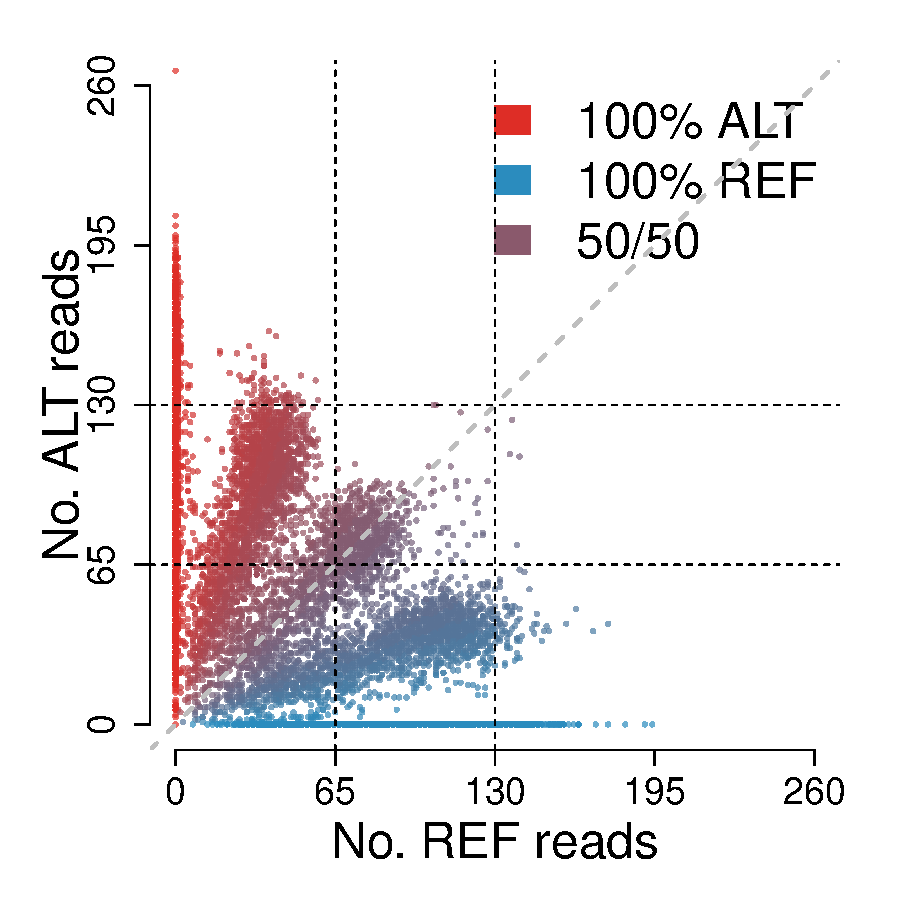
\includegraphics[width=0.3\textwidth]{altVsRef.pdf}}
  \subfloat[][]{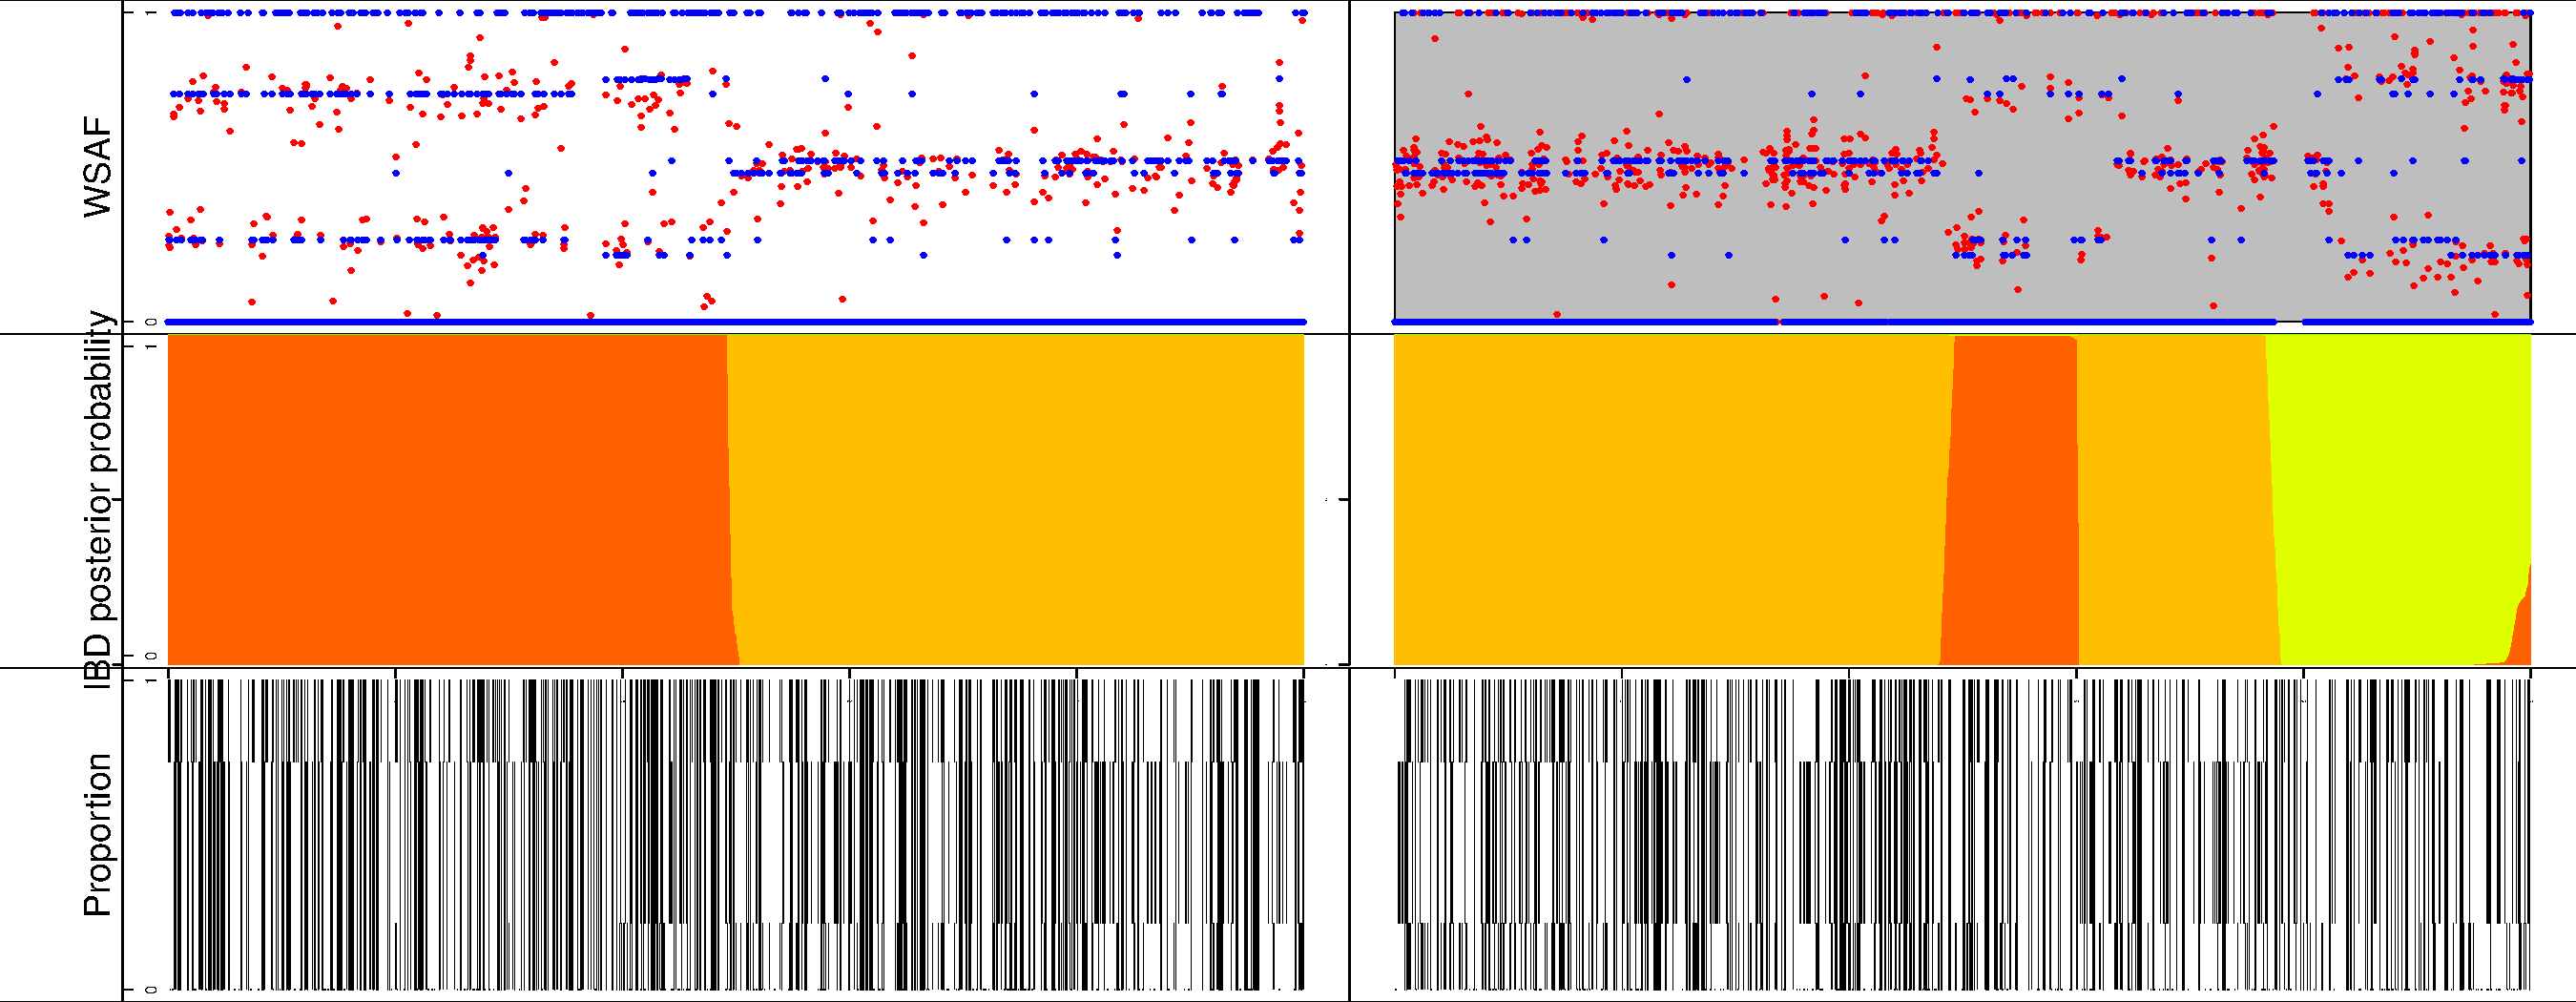
\includegraphics[width=0.7\textwidth]{hap_post_prob_hap.pdf}}
   \caption{{\fontsize{9}{10.8}\selectfont This is font 9} {\fontsize{8}{9.6}\selectfont This is font 8} {\fontsize{6}{7.2}\selectfont This is font 6}
   Deconvolution of field sample PD0577-C from Thailand.  (a) Summary of allele frequencies observed within the isolate shown as a scatter-plot of the numbers of reads supporting the reference (REF: x-axis) and alternative (ALT: y-axis) alleles. (b) The profile of within-sample allele frequency along chromosomes 11 and 12 (black points) suggests a changing profile of IBD with three distinct strains, estimated to be at frequencies of $22\%$, $52\%$ and $26\%$ respectively (other chromosomes omitted for clarity, see Figure~\ref{fig:fig1}-Supplement~1); blue points indicate expected allele frequencies within the isolate.  However, the strains are inferred to be siblings of each other: green segments identify where all three strains are IBD; yellow, orange and dark orange segments identify the regions where one pair of strains are IBD but the others are not.  In no region are all three strains inferred to be distinct. A graphical description of the modules and work flows for \texttt{DEploidIBD} is given in Figure~\ref{fig:fig1}-Supplement~2.}\label{fig:fig1}
   \end{center}
   \figsupp{Whole genome deconvolution of field sample PD0577-C is represented in ring figures. The outer ring show expected WSAF (blue) and observed WSAF (red) across the genome. Red and blue points indicate observed and expected allele frequencies within the isolate. This inner ring marks the IBD regions of the three strains: green segments identify where all three strains are IBD; yellow, orange and dark orange segments identify the regions where one pair of strains are IBD but the others are not.  In no region are all three strains inferred to be distinct.}{\includegraphics[width=.7\textwidth]{{myring.ring}.pdf}}
   \figsupp{A graphical description of the modules and work flows for \texttt{DEploidIBD}.}{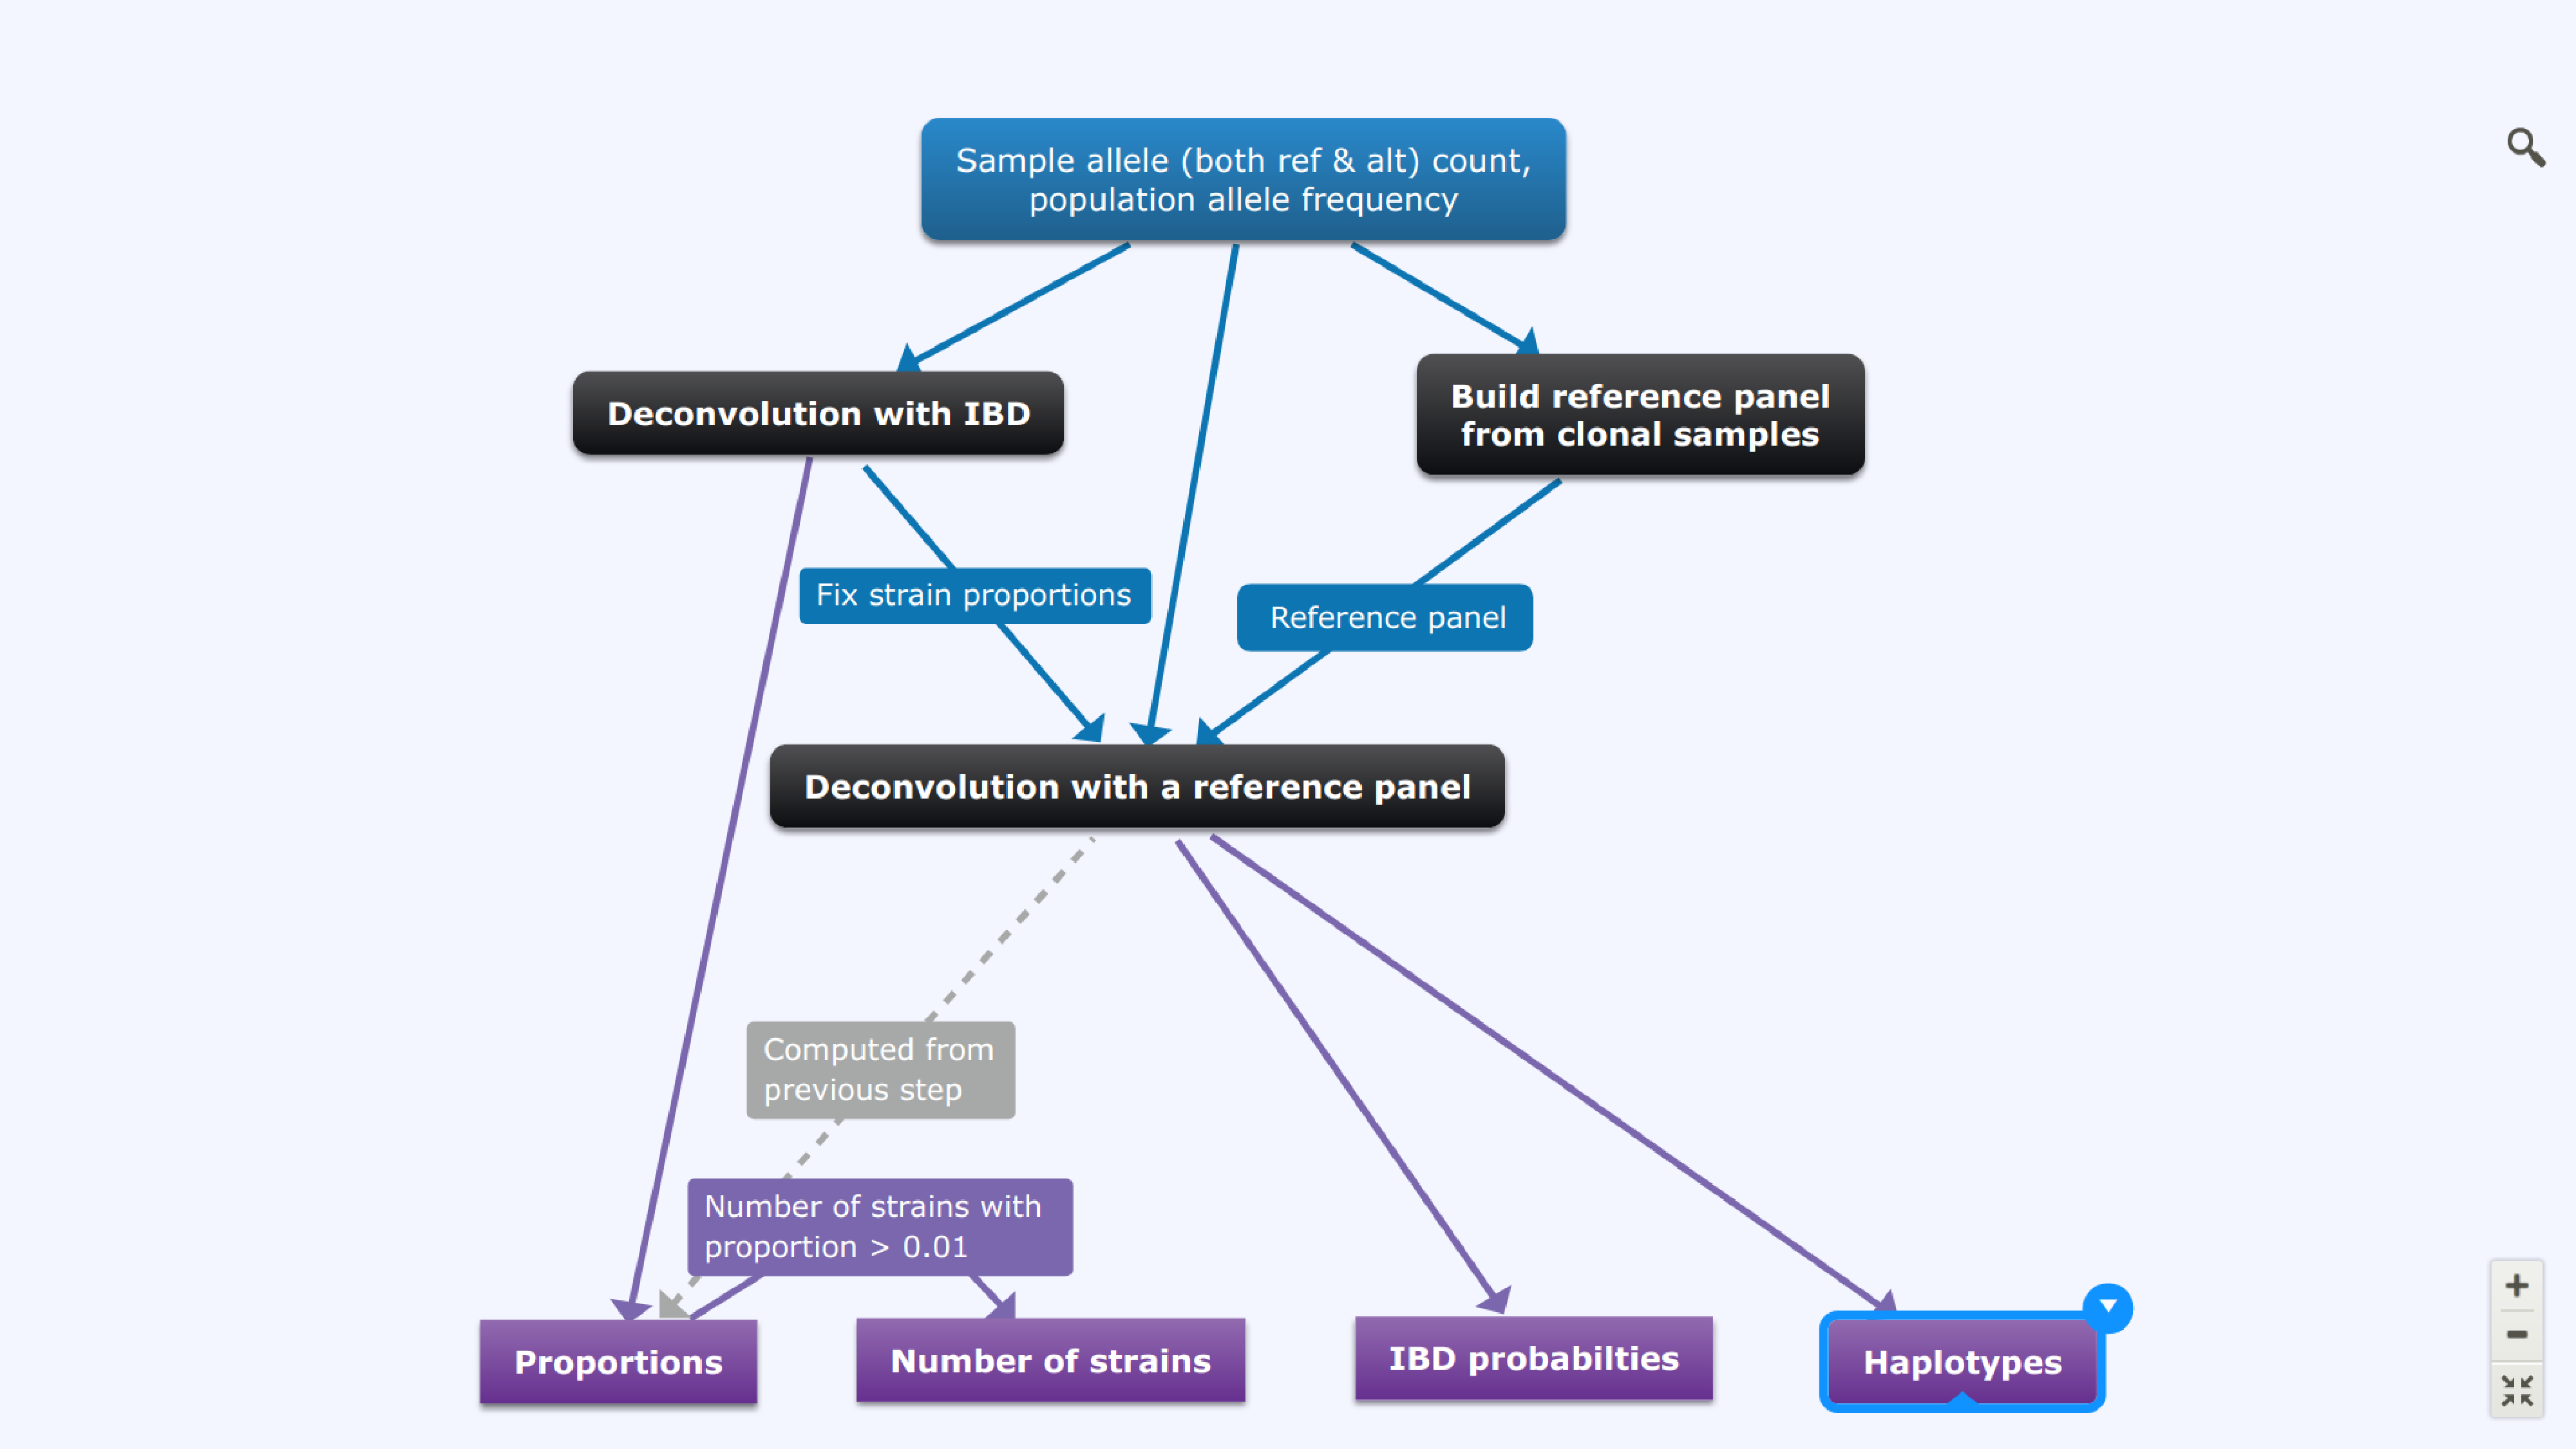
\includegraphics[width=.8\textwidth]{scheme.pdf}}
\end{figure}

\begin{figure}[ht]
  \begin{center}
  \subfloat[][]{\includegraphics[width=0.6\textwidth]{figure_a.pdf}}
  \subfloat[][]{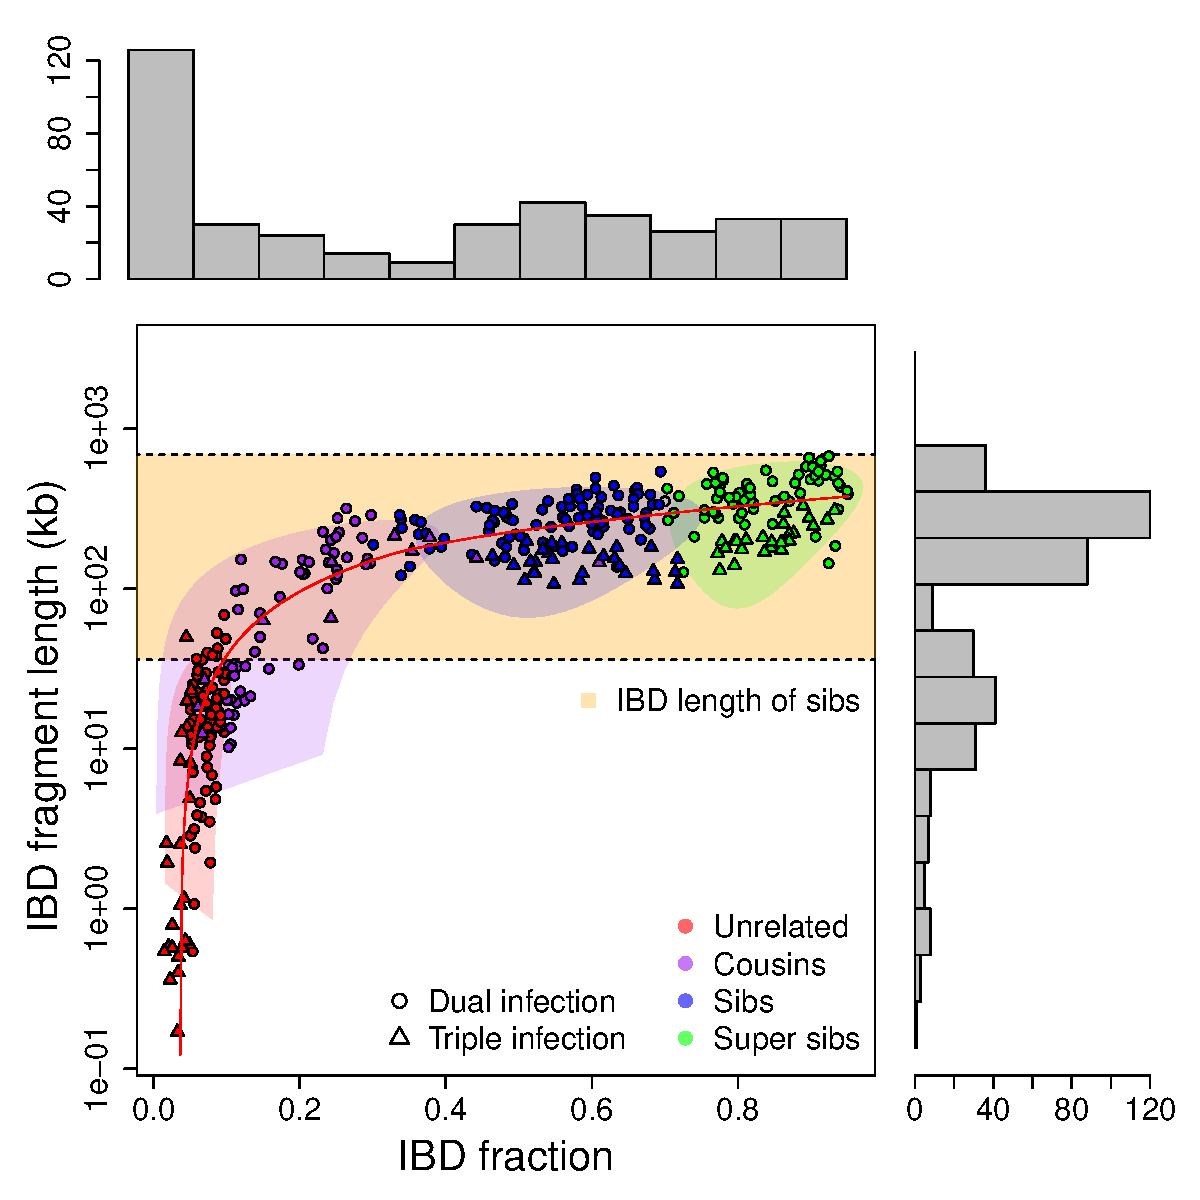
\includegraphics[width=.4\textwidth]{figure_b.pdf}}
   \caption{}\label{fig:fig_unnumberd}
   \end{center}
   \figsupp{IBD chunk lengths from crosses.}{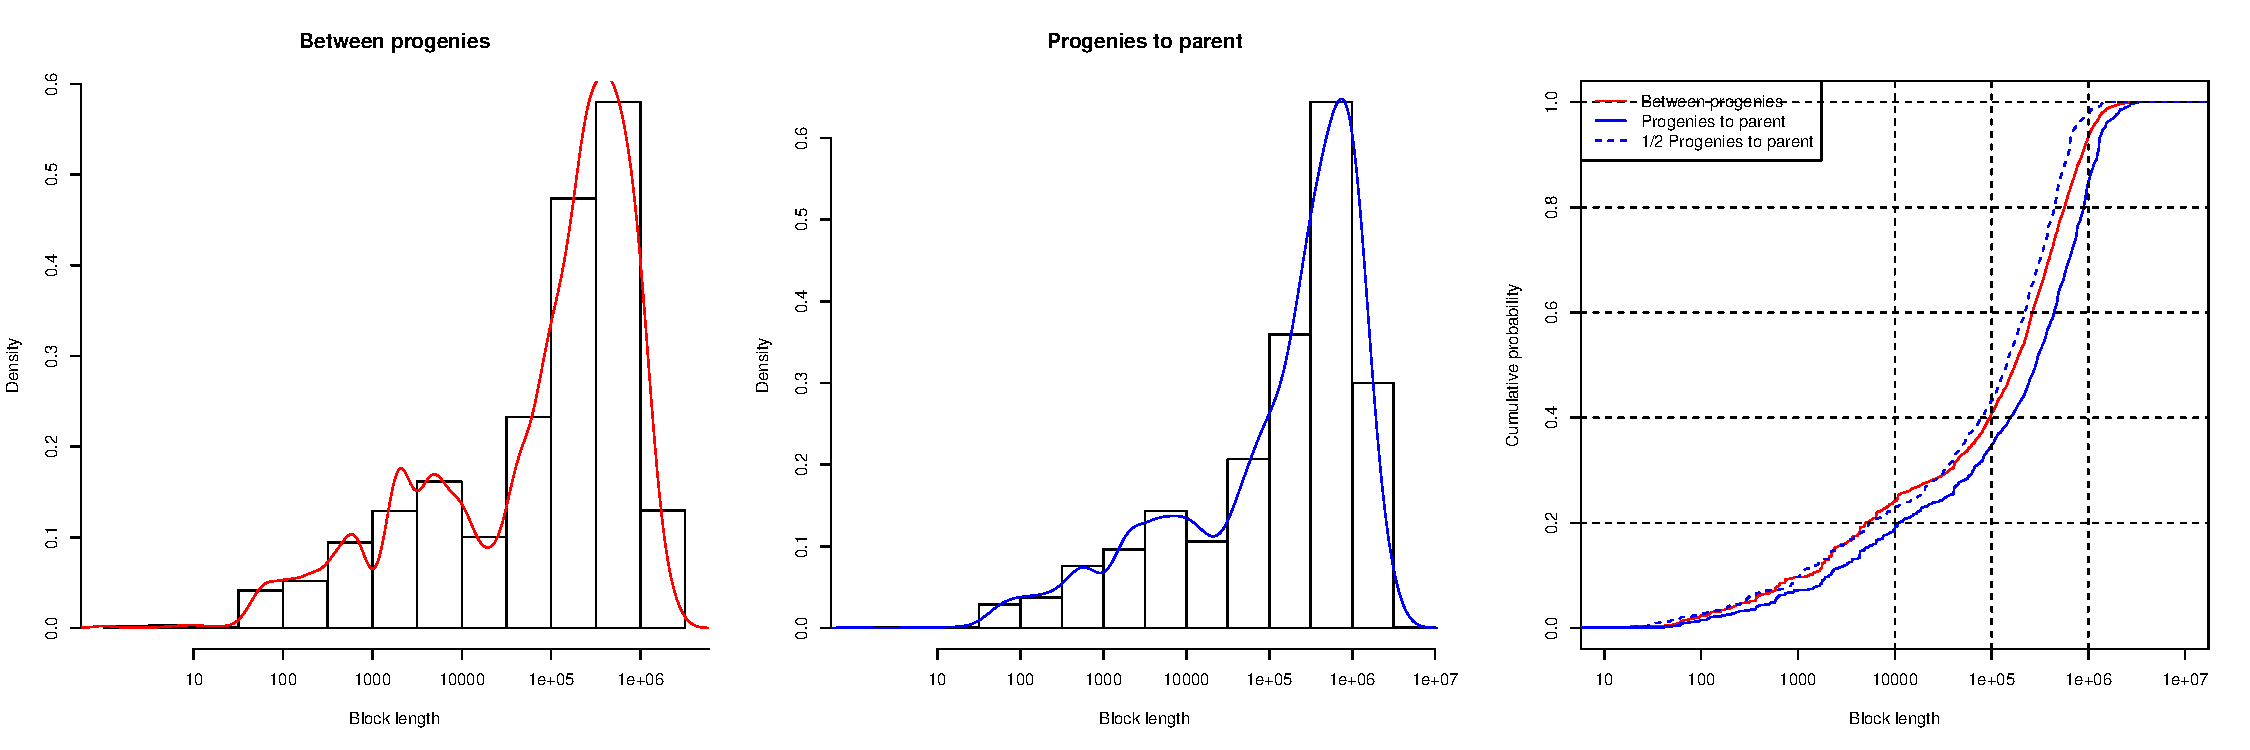
\includegraphics[width=\textwidth]{crosses_IBD_length.pdf}}
\end{figure}


\subsection{Validation}

We validated \texttt{DEploidIBD} through two experiments.  First, to test consistency with \texttt{DEploid} \citet{Zhu2017}, we re-analysed the 27 experimental mixtures from \citep{Wendler2015}.  This data set includes 27 samples of various mixtures of four laboratory parasite lines (3D7, Dd2, HB3 and 7G8; Figure \ref{fig:benchmark} – figure supplement 1).  Allowing for mixtures of up to four strains and using optimal reference panels, we found comparable performance with the single-step \texttt{DEploid} method, with the exception of three strains of equal proportions where LD info is necessary to achieve accurate deconvolution (Figure \ref{fig:benchmark}).

To test the performance of \texttt{DEploidIBD} in a more realistic setting, we created {\it in silico} mixtures from 212 clonal samples of Asian origin with two proportions (25/75\% and 45/55\%) for 8071 sites from Chromosome 14.  A further 20 randomly chosen samples were used as the reference panel. In order to compare the performance of the two methods at different levels of relatedness, we set 25\%, 50\% and 75\% of the second haplotype to be the same as the first haplotype to mimic scenarios of low, medium and high relatedness. To simulate data, we used empirical read depths and drew read counts for the two alleles from binomial proportions.  We inferred strain proportions (summarised by the effective number of strains: $1/\sum w_{i}^{2}$), and haplotypes.  Both \texttt{DEploid} and \texttt{DEploidIBD} correctly estimate strain proportions with low to moderate relatedness and high coverage.  However, for samples with closely related strains, particularly at low coverage, only \texttt{DEploidIBD} can identify the correct number of strains and their proportions.  Genotype and phase errors are comparable between methods, though decrease with increasing relatedness due to the increased homozygosity.  In summary, joint inference of IBD profiles and strain haplotypes is expected to improve estimates of strain proportions (and hence haplotypes), particularly in regions with high rates of IBD and with low sequencing coverage.  Moreover, direct estimates of IBD within mixed infections can be used as additional characterisation of samples.



\begin{figure}[htp]
  \begin{center}
  \subfloat[][]{
  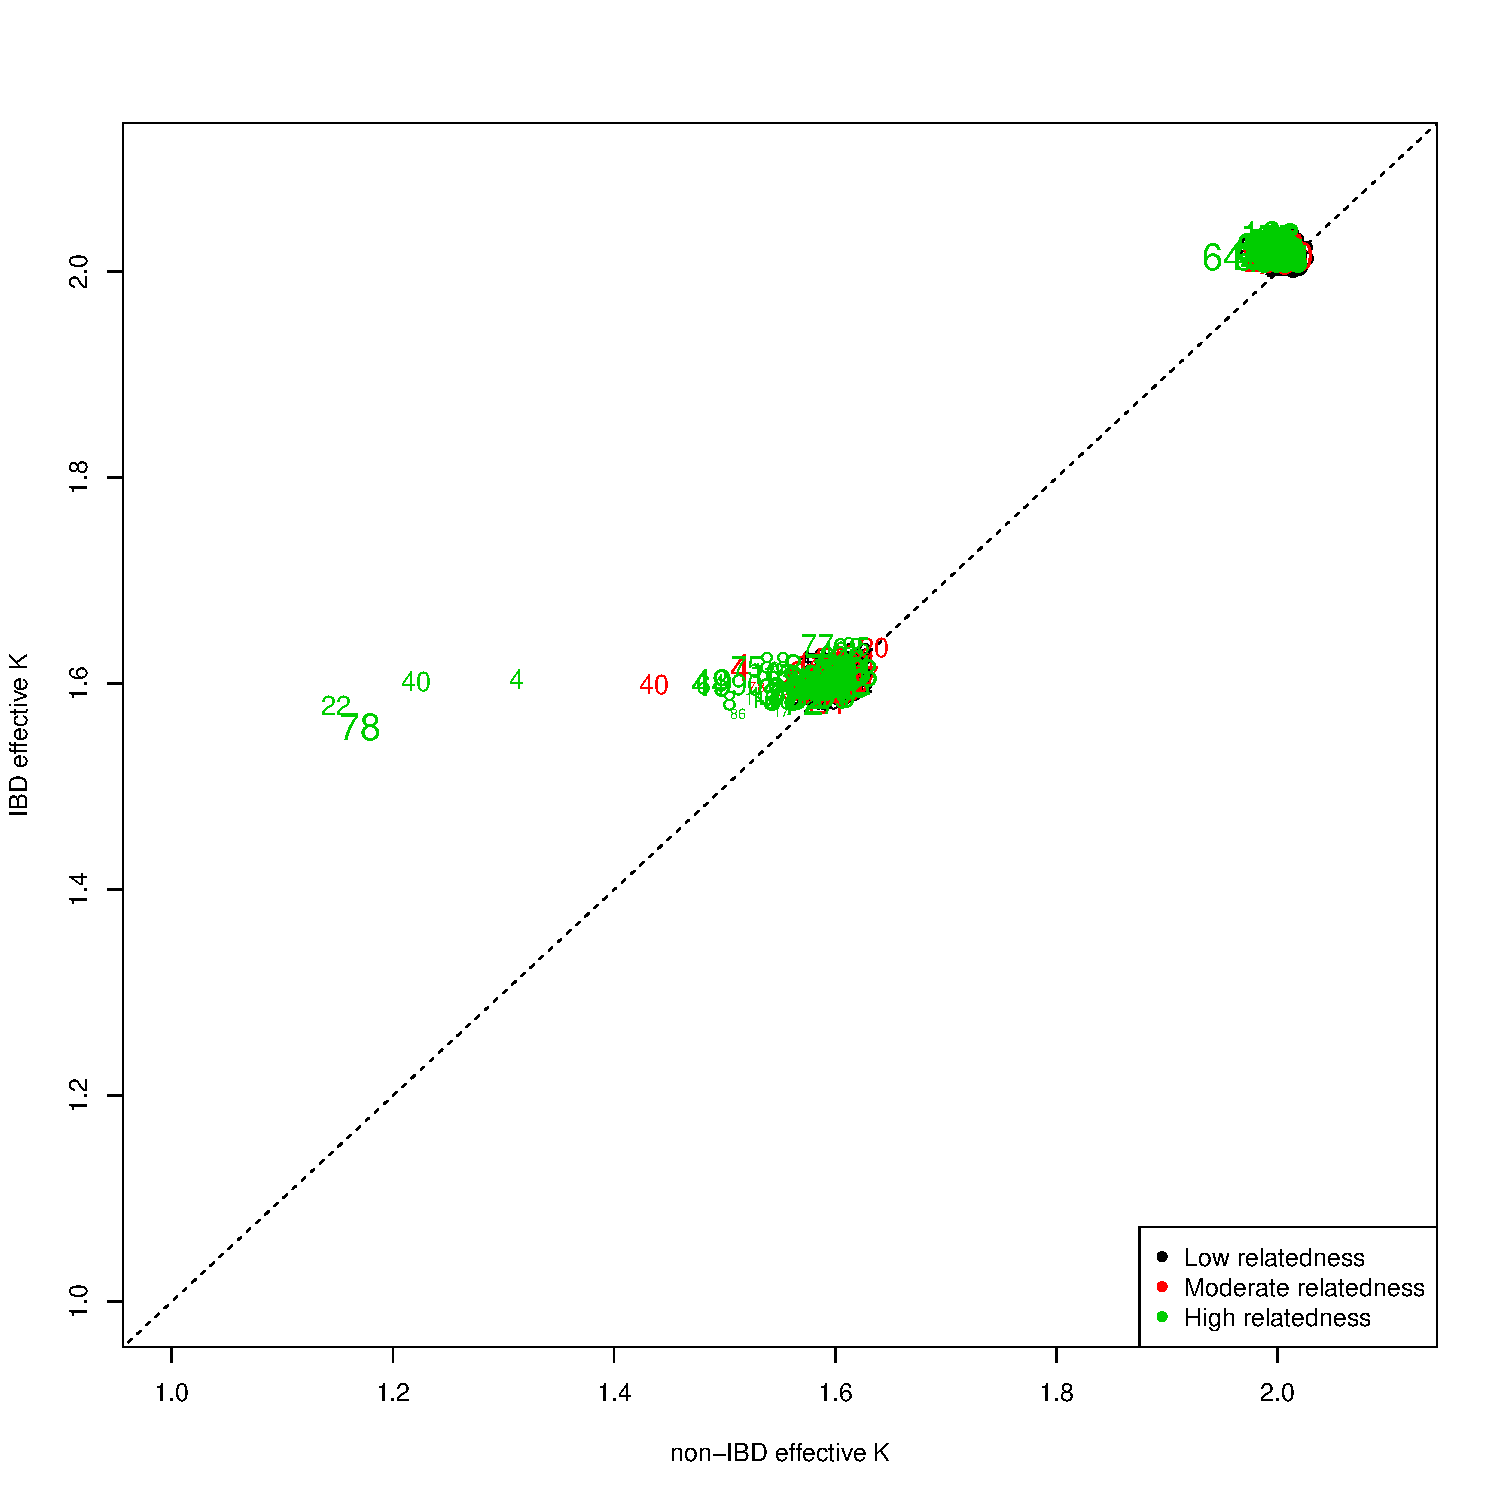
\includegraphics[width = 0.3\textwidth]{diagnositicPlot_of_effK_final.pdf}
  }
  \subfloat[][]{
  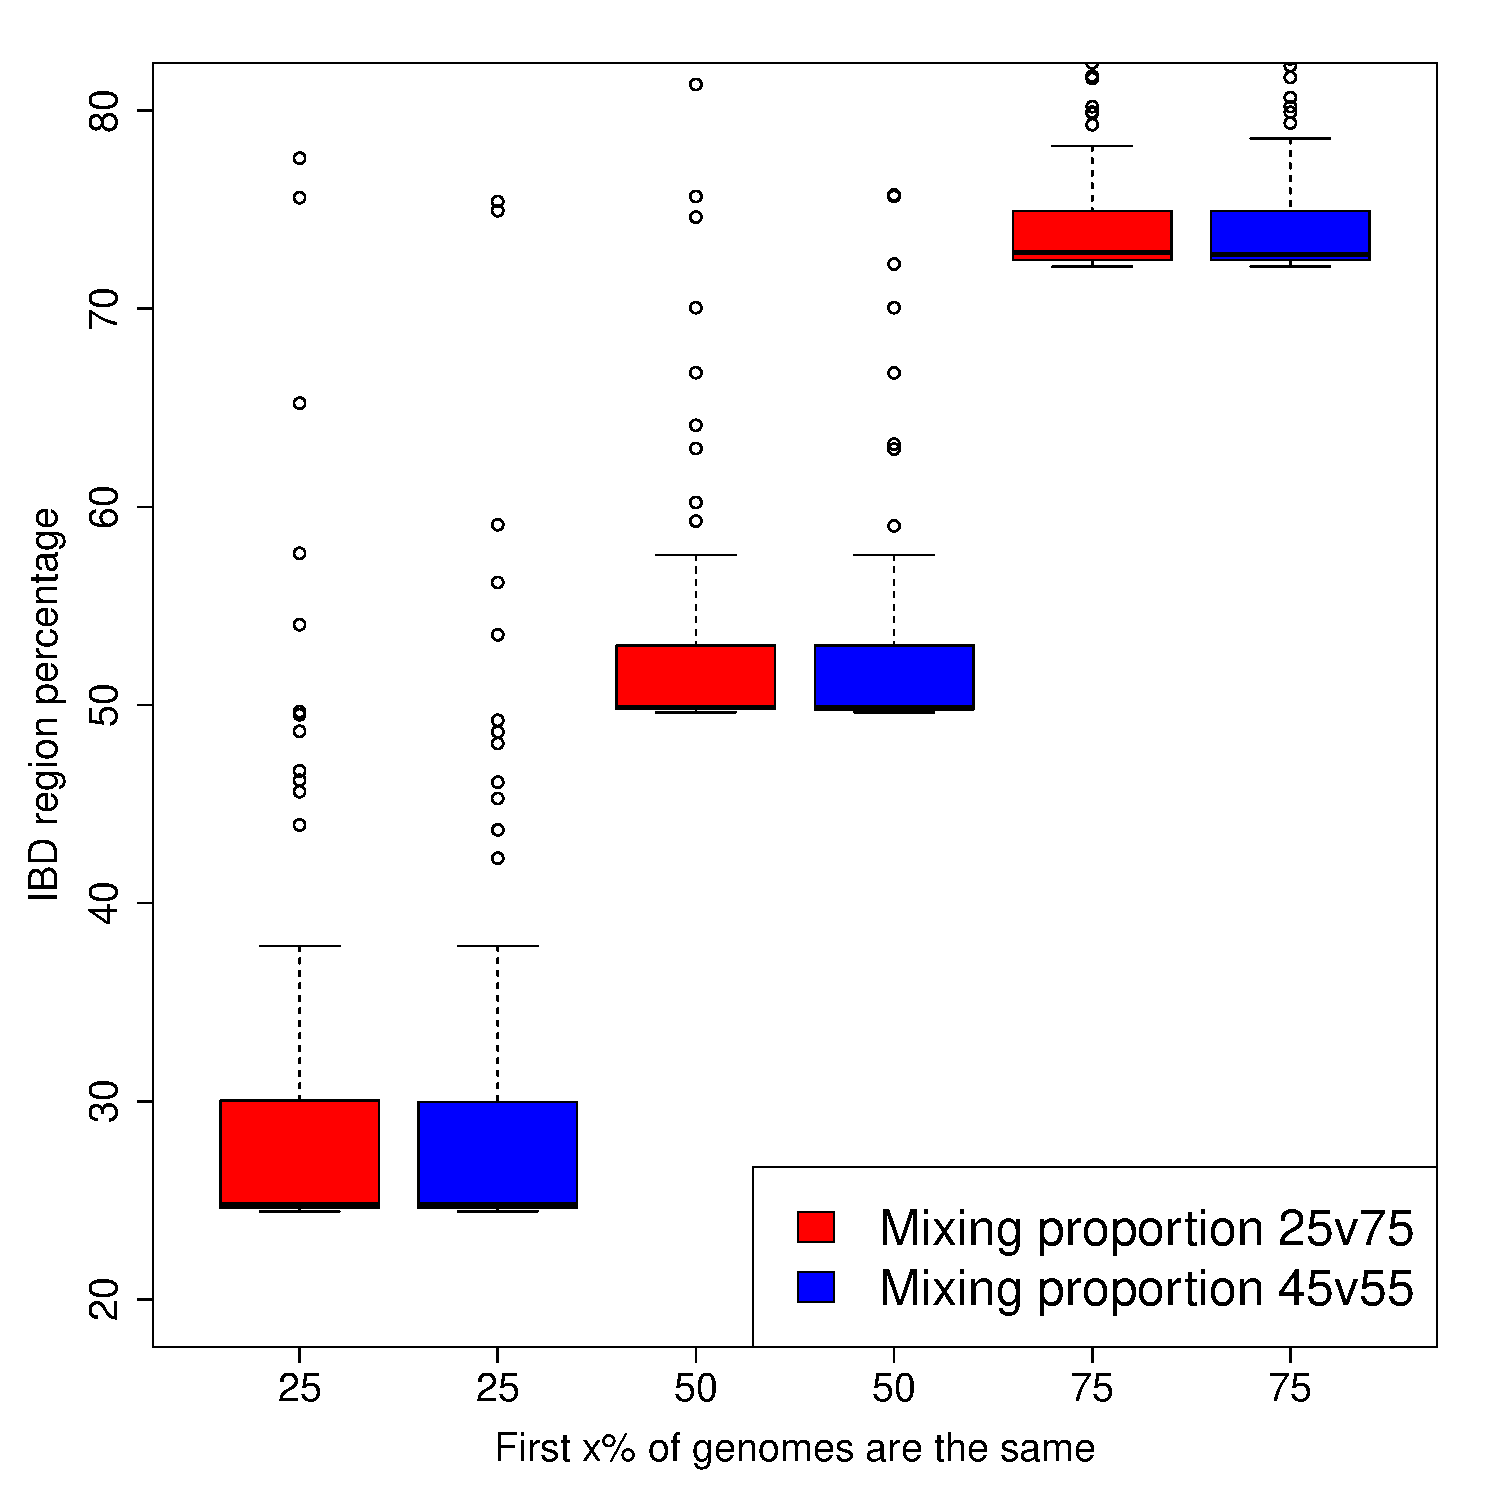
\includegraphics[width = 0.3\textwidth]{IBDprobs.pdf}
  }\\
  \subfloat[][]{
  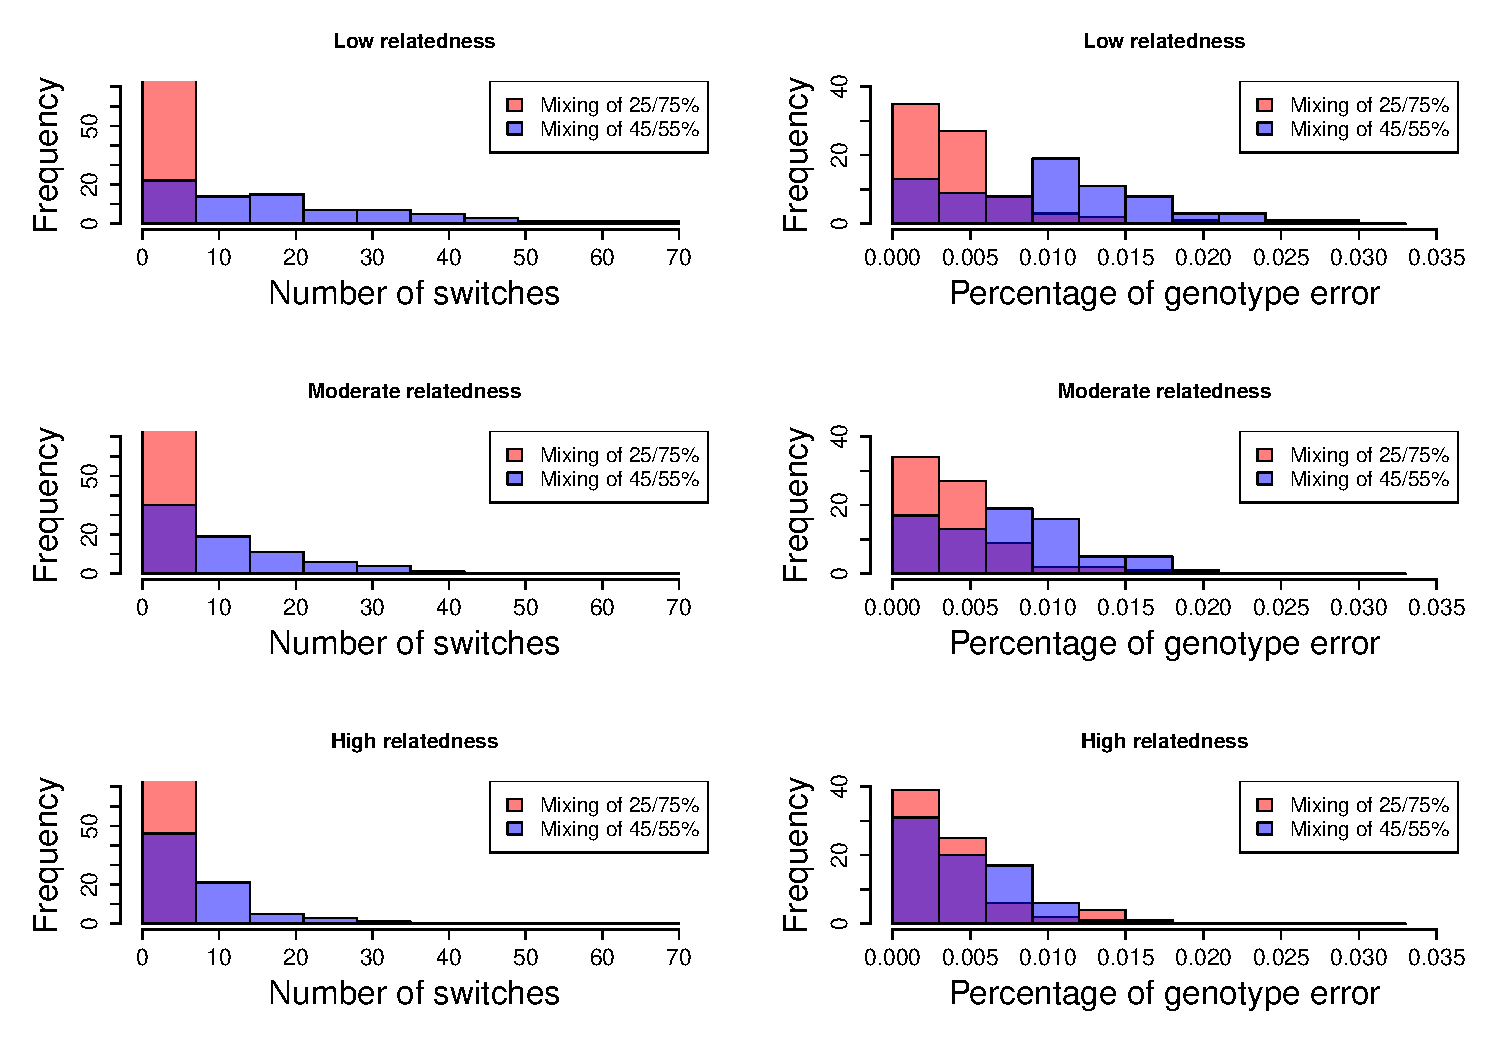
\includegraphics[width = 0.5\textwidth]{IBDHapError.pdf}
  }
  \caption{Simulation results. (a)Comparison of effective number of strains between \texttt{DEploid} and \texttt{DEploidIBD}. (b)Expected and inferred percentage of IBD regions for \texttt{DEploid}. (c) Histograms of switch error and genotype error across 76 simulated Pf3k samples for \texttt{DEploid}. In all figures, we excluded eight cases out of the 100 experiments where simulated haplotypes were over 99\% identical, and 16 cases where average coverage was below 20.
}\label{fig:benchmark}
  \end{center}
  \figsupp{Experimental validation and effective number of strains inferred by {\tt DEploidIBD}. We use a reference panel of the laboratory parasite lines (3D7, Dd2, HB3 and 7G8) to deconvolve the same lab-mixed samples, assuming 3 and 4 strains within a sample. Each experiment is repeated without IBD method. Black crosses indicate the true effective number of strains. Purple crosses indicate median values obtained from 30 replicates when using {\tt DEploidIBD} with a panel and assuming that the maximum number of strains is 4. The coloured dots show the inferred effective number of strains across replicates with intensity proportional to fraction.
  }{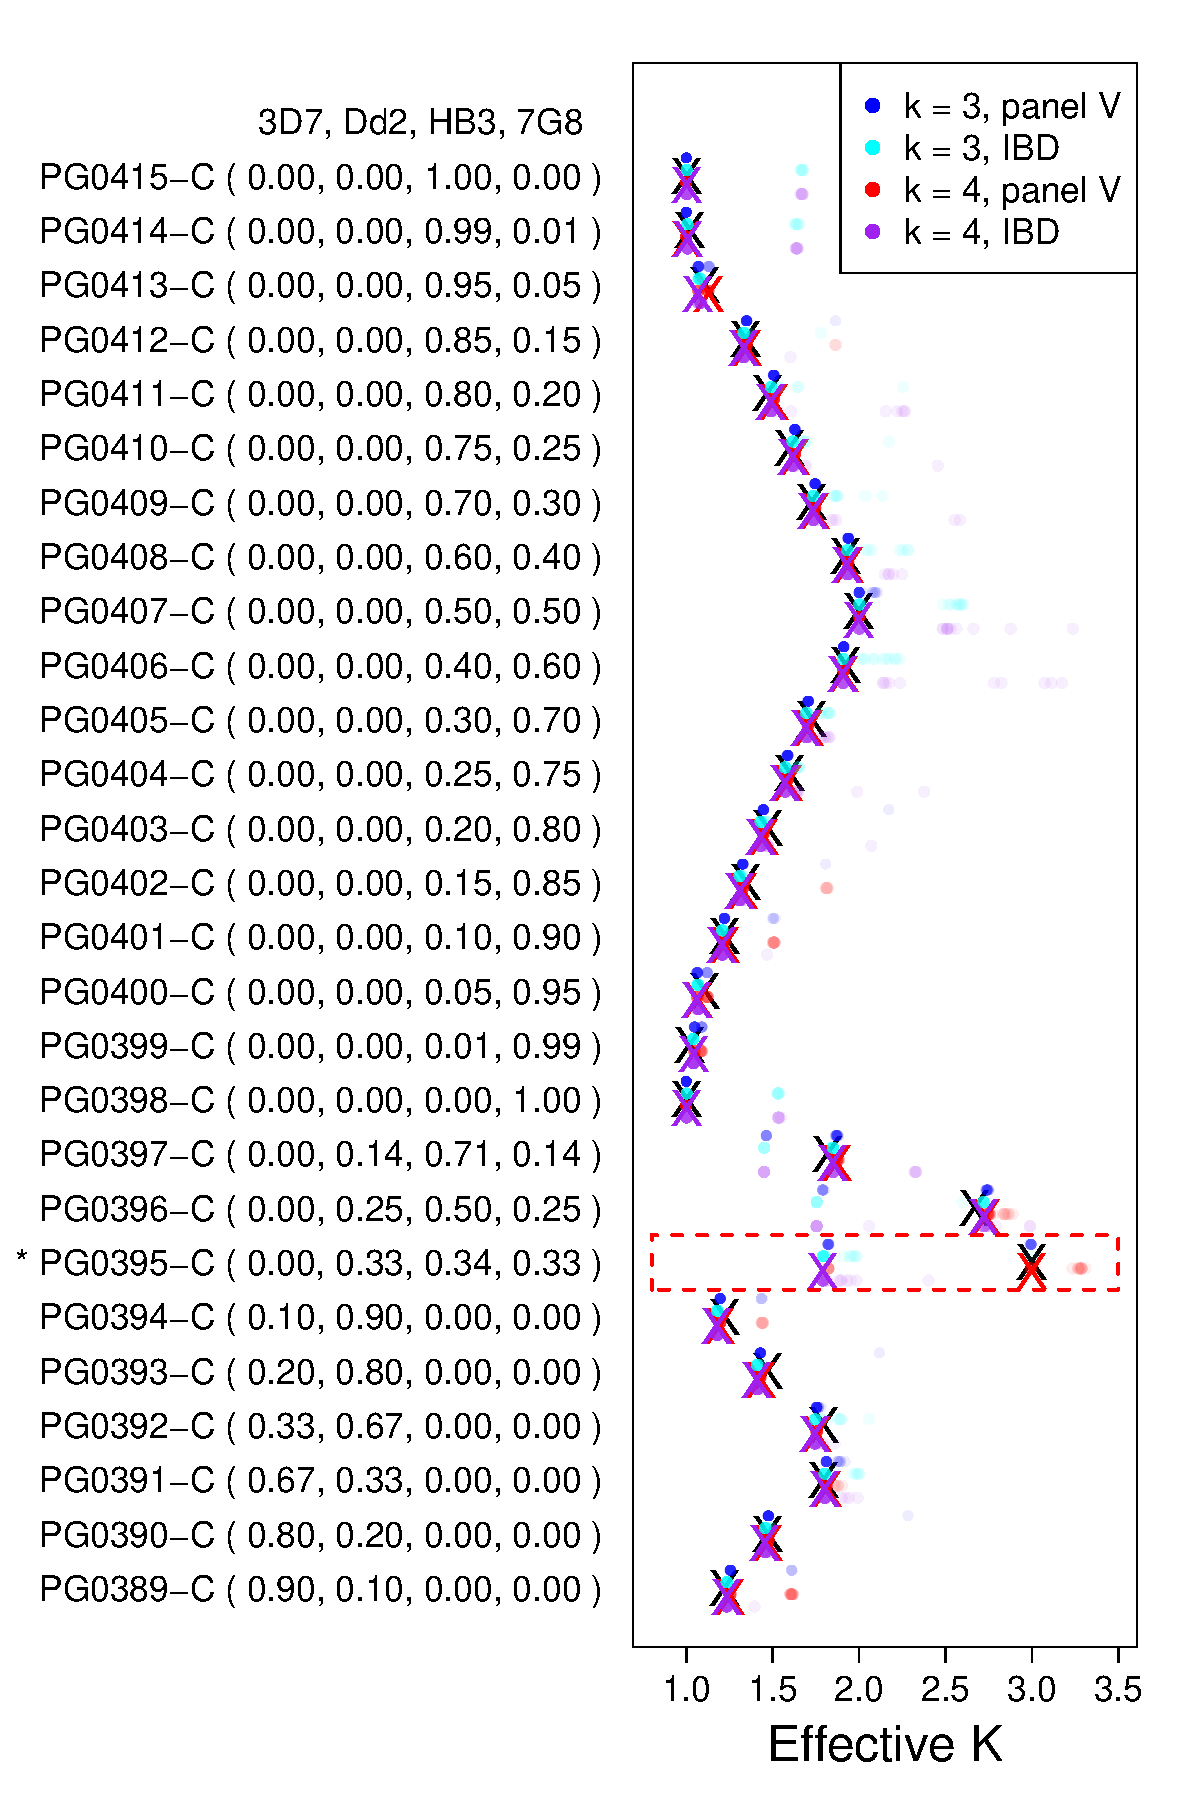
\includegraphics[width = 0.65\textwidth]{eff_k_both.pdf}}
  \figsupp{Comparison of true and inferred haplotypes for Chromosome 14 (2,369 SNPs) in sample PG0396-C before and after haplotype painting using a reference panel of the laboratory parasite lines (3D7, Dd2, HB3 and 7G8). The yellow, cyan and white background label the haplotype segments from strains 7G8, HB3 and Dd2 respectively. The switch errors are obtained by counting the changes of a strain segment mapped to reference strains; the genotype errors are the discordance between the strain and the mapped reference segments. }{\includegraphics[width = 0.8\textwidth]{DEploid_IBD_haps_compare.pdf}}
\end{figure}




\section{Results}

\subsection{The rate and structure of mixed infection in 2,512 {\it P. falciparum} field samples from 14 countries}

To investigate how the rate and relatedness structure of mixed infections varies among geographical regions with different epidemiological characteristics, we applied \texttt{DEploidIBD} to 2,512 field samples of {\it P. falciparum} released by the Pf3k Consortium (REF).  These samples were collected under a wide range of designs, though the majority were taken from individuals seeking treatment for malaria symptoms.  A summary of the data sources is presented in Table \ref{tab:Pf3ksamples}.  After variant calling and filtering, we genotyped approximately 1M variable SNP positions across all samples, sequenced to an average depth of 86 (range 1.0 – 680).  See Supplementary Material for details of filters and data availability.  Samples were grouped into four geographical regions within Africa and three within Asia based on genetic similarity (Table~\ref{tab:Pf3ksamples }).

\begin{table}[bt]
  \caption{Summary of African samples.}\label{tab:Pf3ksamples}
\begin{tabular}{l l c c c c c}
\toprule
Country & Location & Year & Sample size & Mean Read Depth (s.e.) & Group \\
\midrule
Malawi          &Chikwawa       &2011 &208  &97   (3.2 )&Africa 1\\
%                &               &NA   &92   &94   (3.5 )&Africa 1\\
                &               &2012 &10   &133  (9.7 )&Africa 1\\
                &               &2014 &7    &128  (3.1 )&Africa 1\\
                &Zomba          &2011 &34   &88   (9.4 )&Africa 1\\
%                &               &NA   &17   &50   (7.5 )&Africa 1\\
%                &               &2012 &1    &91   (NA  )&Africa 1\\
 \hline
DR of the Congo &Kinshasa       &2013 &113  &49   (3.2 )&Africa 1\\
 \hline
Ghana           &Kassena        &2009 &121  &82   (5.5 )&Africa 2\\
%                &               &NA   &28   &218  (34.5)&Africa 2\\
                &               &2010 &173  &103  (8.6 )&Africa 2\\
                &               &2011 &96   &72   (4.3 )&Africa 2\\
                &               &2012 &39   &110  (4.4 )&Africa 2\\
                &               &2013 &92   &114  (4.5 )&Africa 2\\
                &Kintampo       &2011 &7    &86   (11.8)&Africa 4\\
 %               &               &NA   &20   &107  (17  )&Africa 4\\
                &               &2012 &38   &143  (9.5 )&Africa 4\\
                &               &2013 &3    &165  (53.4)&Africa 4\\
 \hline
Mali            &Kolle          &2007 &51   &82   (10.5)&Africa 3\\
                &Faladje        &2007 &36   &75   (10.1)&Africa 3\\
                &Bandiagara     &2007 &9    &95   (25.2)&Africa 3\\
 \hline
Nigeria         &               &2012 &4    &51   (20.9)&Africa 3\\
%               &Ilorin         &2011 &1    &39   (NA  )&Africa 3\\

 \hline
Senegal         &Thies          &2002 &5    &60   (7.8 )&Africa 3\\
                &               &2004 &2    &130  (68.2)&Africa 3\\
%                &               &2001 &1    &59   (NA  )&Africa 3\\
                &               &2008 &22   &94   (4.9 )&Africa 3\\
                &               &2011 &32   &97   (6   )&Africa 3\\
                &               &2007 &4    &83   (9   )&Africa 3\\
                &               &2009 &43   &175  (14.9)&Africa 3\\
                &               &2010 &24   &159  (9.7 )&Africa 3\\
                &Velingara      &2004 &2    &56   (2.2 )&Africa 3\\
                &               &2005 &2    &71   (4   )&Africa 3\\
 \hline
The Gambia      &GM\_Coastal    &2008 &65   &129  (9.4 )&Africa 4\\
 \hline
Guinea          &Nzerekore      &2011 &100  &75   (4.5 )&Africa 4\\
\bottomrule
\end{tabular}

\medskip
Source: \url{ftp://ngs.sanger.ac.uk/production/pf3k/release_5/5.1}

\tabledata{Pf3k data release 5.1 contains a set of {\em de novo} genotypes for the 5.0 sample set. The genotyping, including both indel and SNP variants, was performed using a pipeline based on GATK best practices.}
\end{table}

\begin{table}[bt]
\ContinuedFloat
\caption{Table continued.  Summary of Asian samples.}
\begin{tabular}{l l c c c c c}
\toprule
Country & Location & Year & Sample size & Read Depth (s.e.) & Group \\
\midrule
Thailand        &Sisakhet       &2011 &5    &112  (25.4)&Asia 1  \\
                &               &2012 &13   &89   (13  )&Asia 1  \\
                &               &2013 &4    &57   (7.8 )&Asia 1  \\
                &Mae Sot        &2011 &37   &67   (7.3 )&Asia 3  \\
                &               &2012 &69   &83   (4.9 )&Asia 3  \\
                &Ranong         &2011 &9    &96   (18.4)&Asia 3  \\
                &               &2012 &11   &82   (12.4)&Asia 3  \\
 \hline
Cambodia        &Pursat         &2009 &18   &75   (9.3 )&Asia 1  \\
                &               &2010 &101  &91   (5.2 )&Asia 1  \\
%                &               &NA   &5    &181  (97.2)&Asia 1  \\
                &               &2011 &104  &48   (3   )&Asia 1  \\
                &               &2012 &7    &37   (19.1)&Asia 1  \\
                &Pailin         &2011 &50   &53   (4.1 )&Asia 1  \\
                &               &2012 &34   &46   (5.2 )&Asia 1  \\
                &Ratanakiri     &2010 &50   &71   (6.1 )&Asia 2  \\
                &               &2011 &82   &45   (4.2 )&Asia 2  \\
                &               &2012 &15   &44   (8.9 )&Asia 2  \\
                &Preah Vihear   &2011 &75   &51   (5.2 )&Asia 2  \\
                &               &2012 &29   &45   (6.8 )&Asia 2  \\
 \hline
Vietnam         &Phuoc Long     &2011 &27   &68   (7.2 )&Asia 2  \\
                &               &2012 &5    &107  (6.3 )&Asia 2  \\
                &Bu Gia Map     &2011 &44   &66   (5   )&Asia 2  \\
                &               &2012 &20   &110  (8.7 )&Asia 2  \\
%                &Bu Dang        &2011 &1    &94   (NA  )&Asia 2  \\
 \hline
Laos            &Attapeu        &2011 &59   &71   (4.2 )&Asia 2  \\
                &               &2012 &26   &77   (7   )&Asia 2  \\
 \hline
Myanmar         &Bago Division  &2011 &12   &59   (7.1 )&Asia 3  \\
                &               &2012 &47   &62   (5.2 )&Asia 3  \\
%                &               &2013 &1    &27   (NA  )&Asia 3  \\
 \hline
Bangladesh      &Ramu           &2012 &50   &53   (4.2 )&Asia 3  \\
\bottomrule
\end{tabular}
\end{table}

Across continents and countries we find substantial variation in the rate and relatedness structure of mixed infections (Figure~\ref{fig:Pf3kResults}).  Within Africa, rates of mixed infection vary from 18\% in Senegal to 63\% in Malawi.  In the South East Asian field samples, mixed infection rates are generally lower, though also vary considerably; between 22\% in Thailand to 56\% in Bangladesh.  Where data for a location is available over multiple years, we find little evidence for substantial fluctuation over time CHECK .  Between 5.1\% (Senegal) and 40\% (Malawi) of individuals have more than two strains present and, at the population level, there is a positive correlation between the rate of dual infection (where two strains are present) and higher levels of infection (linear model P = 0.017, accounting for continental level effects). 

Relatedness between samples and populations also varied substantially (Figure~\ref{fig:Pf3kResults}).  In dual infections, the average fraction of the genome inferred to be IBD ranges from 16\% in Guinea to 55\% in The Gambia and Asian populations show on average a higher level of relatedness (41\%) compared to African populations (30\%).  Similarly, while a minority of triple infections (0\% to 24\% across populations) are estimated to be unrelated in Africa, all triple Asian infections are inferred to contain individuals related at the level of at least siblings.  Overall, 58\% of all mixed infections involve strains with over 30\% of the genome IBD (the 2.5th percentile of IBD expected between true siblings given the recombination rate in {\it P. falciparum}).  


Within both Africa and Asia we find no simple relationship between IBD and rates of mixed infection (Figure~\ref{fig:Pf3kResults}).  In both Africa and Asia, the populations with the highest levels of mixed infection have between 40\% and 60\% of strains with highly related (IBD fraction $\gt 0.3$) strains.  However, similar patterns are observed across all populations.  Moreover, populations with similar rates of mixed infection can have different patterns of inbreeding.  For example, Senegal, which has low rates of mixed infection, has relatively low levels of IBD (VALUE) where mixed infections occur, while The Gambia, which has only slightly higher rates of mixed infection has considerably higher levels of IBD (VALUE).  




\begin{figure}[htp]
  \centering{}
  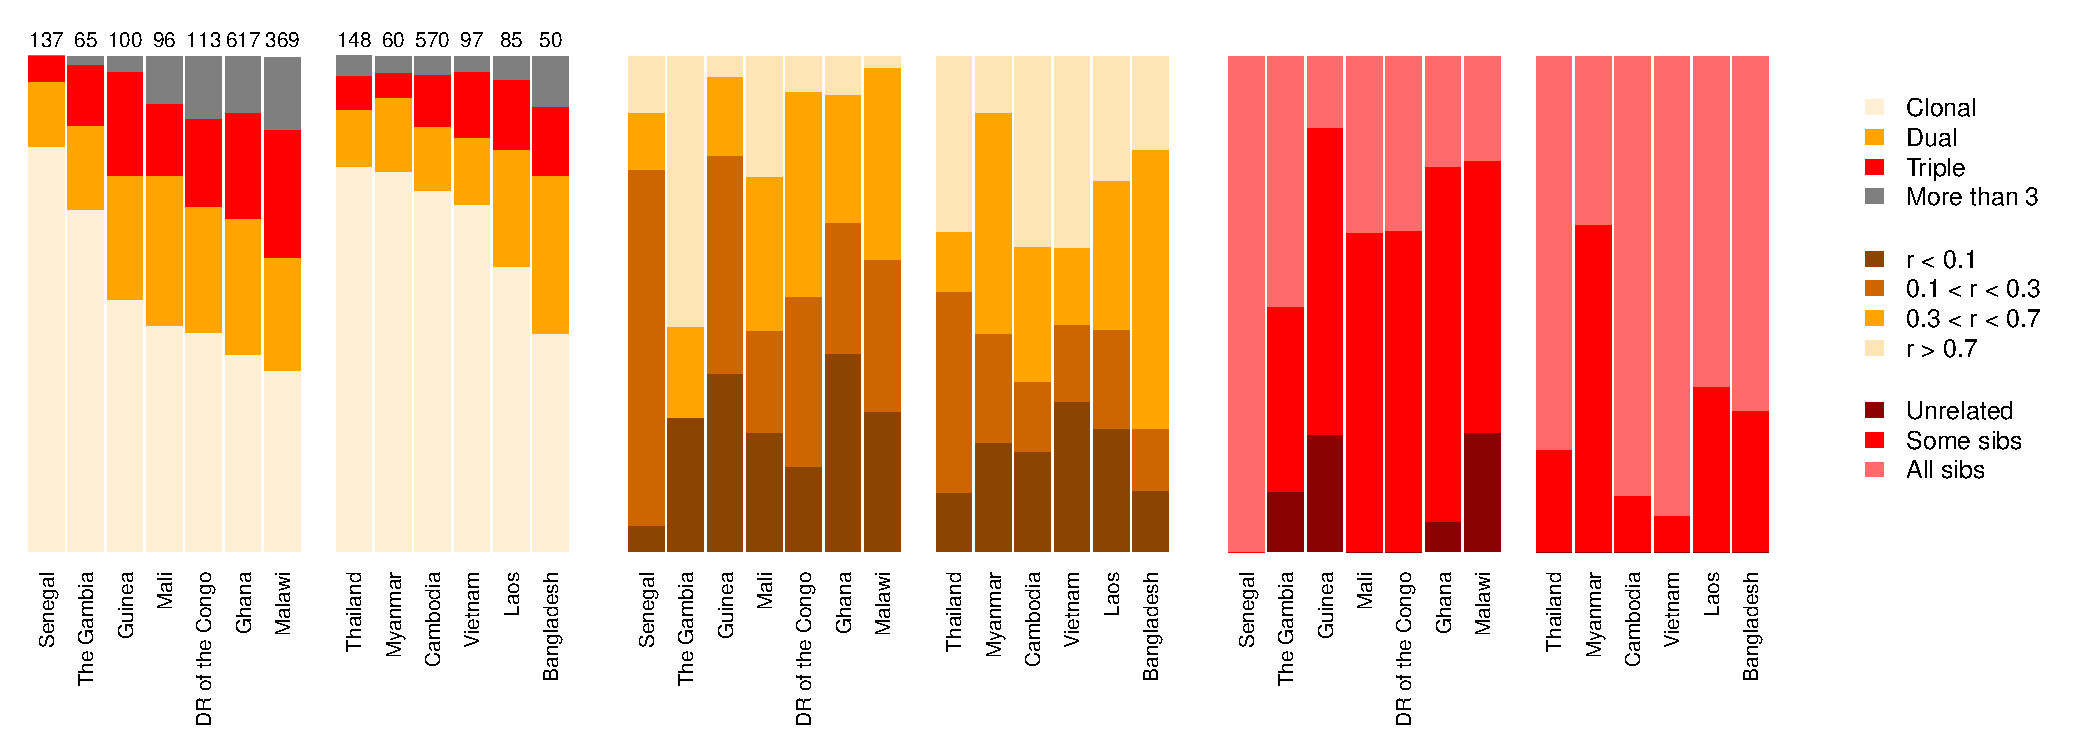
\includegraphics[width=\textwidth]{barPlots_by_gil.pdf}
  \caption{tmp}\label{fig:Pf3kResults}
\end{figure}






\subsection{Inferring genealogical relationships between strains within a host}


\subsection{Characterising genealogical relationships at the population level}


\subsection{Characteristics of mixed infection correlate with local pathogen prevalence}


\subsection{A mathematical model of mixed infection}





\subsection{Monitoring malaria epidemic from the IBD configuration probabilities}


We show how the genomes of co-existing strains are related to each other, observing in some cases high levels of genetic relatedness or inbreeding. We see cases where heterozygosity is structured along the genome in a manner that suggests inbreeding, finding multiple cases of strains that are within 1-2 meioses of each other (Fig~\ref{fig:fig1}(a)). We envision that such a signature could be exploited in future micro-epidemiological studies to help in the inference of infection histories and transmission trees.

At the population level, we explore the malaria epidemic by stacking up all IBD posterior probabilities (Fig~\ref{fig:gambia}(a)). We observe striking variation in inbreeding patterns across populations with a mean inbreeding fraction range of \textcolor{red}{[0.07, 0.54]}. African countries, with the exception of The Gambia and Senegal, seem to have less inbred mixed infections, in agreement with the different levels of genetic diversity observed in each continent. These population-specific differences relate to the epidemiological setting of each region and provide a novel, and potentially important, source of information about local infection dynamics.

Between the mixed samples, we computed pairwise correlation between the IBD-fraction across genome. As expected, we observe high correlations in IBD profiles from 22 Malawi samples that had been sequenced twice through the MalariaGEN pipeline. We also observe similar high correlations between unique samples in Vietnam, Gambia, Cambodia and Bangladesh. We used threshold of 0.8 correlation to identify related infections. For example, in Figure~\ref{fig:gambia}(b), two pairs of sample, PA0068-C and PA0069-C, PA0021-C and PA0027-C show very strong correlations between the IBD-fraction across the genome. Samples PA0021-C and PA0027-C show very little evidence of inbreeding. On the other hand, we observe a strong negative correlation between the WSAF, which we speculate that both infections are caused by two mosquito carrying single strain of parasite, but the infection times are different; or one patent had been treated but the effect of drug appear differently, because the dominate strain in PA0021-C is the minor strain of PA0027-C, and vice versa. In the other case, parasite strains within samples PA0068-C and PA0069-C show strong evidence of IBD sharing, which can only happen when two people were bitten by the same mosquito, which is carrying two strains that have recombined within the mosquito. Interestingly, we observe the third strain in PA0068-C, which could mean that recombination is already happening again. Or we just don't observe it in PA0069-C.

%These samples are mixtures of two, with proportions of
%==> PA0021-C_newFilter_seed1_IBD.log <==
  %0.747591    3.23594e-09      0.252409    3.42703e-09

%==> PA0027-C_newFilter_seed1_IBD.log <==
  %0.860842    2.3895e-09      0.139158    2.52997e-09

%==> PA0068-C_newFilter_seed1_IBD.log <==
  %0.783381     0.0387533    4.0773e-05      0.177825

%==> PA0069-C_newFilter_seed1_IBD.log <==
  %0.665359    4.58131e-09      0.334641    4.92958e-09

%On average, two unrelated strains differ at 8000 places, and I found
%#> sum(PA0021.haps$h1 != PA0027.haps$h3)
%#[1] 380
%#> sum(PA0021.haps$h3 != PA0027.haps$h1)
%#[1] 119

%#> sum(PA0068.haps$h1 != PA0068.haps$h4)
%#[1] 820
%#> sum(PA0068.haps$h1 != PA0069.haps$h1)
%#[1] 368
%#> sum(PA0068.haps$h4 != PA0069.haps$h3)
%#[1] 438




\subsection{Malaria prevalence prediction}

We believe that the detailed characterization of mixed infections, in conjunction with localised epidemiological datasets like the ones provided by the Malaria Atlas Project [Bhatt et al., 2015], will improve our understanding of malaria epidemiology across the globe, permitting the identification of the major factors that modulate transmission in different countries. We also foresee that these methods will have important applications on the assessment of on-going interventions via genomic data [Volkman et al., 2012].

\textcolor{red}{update the linear model when cluster finishing }

Independence between effective k and IBD fraction (see Figure~.S*).

\narrative{4. Simulation results to analyse the relationship between prevalence, mixed infection rate and sib-strain rate.  Figure 5 summarising simulations.}


\begin{figure}[htp]
\centering
  \subfloat[][]{
  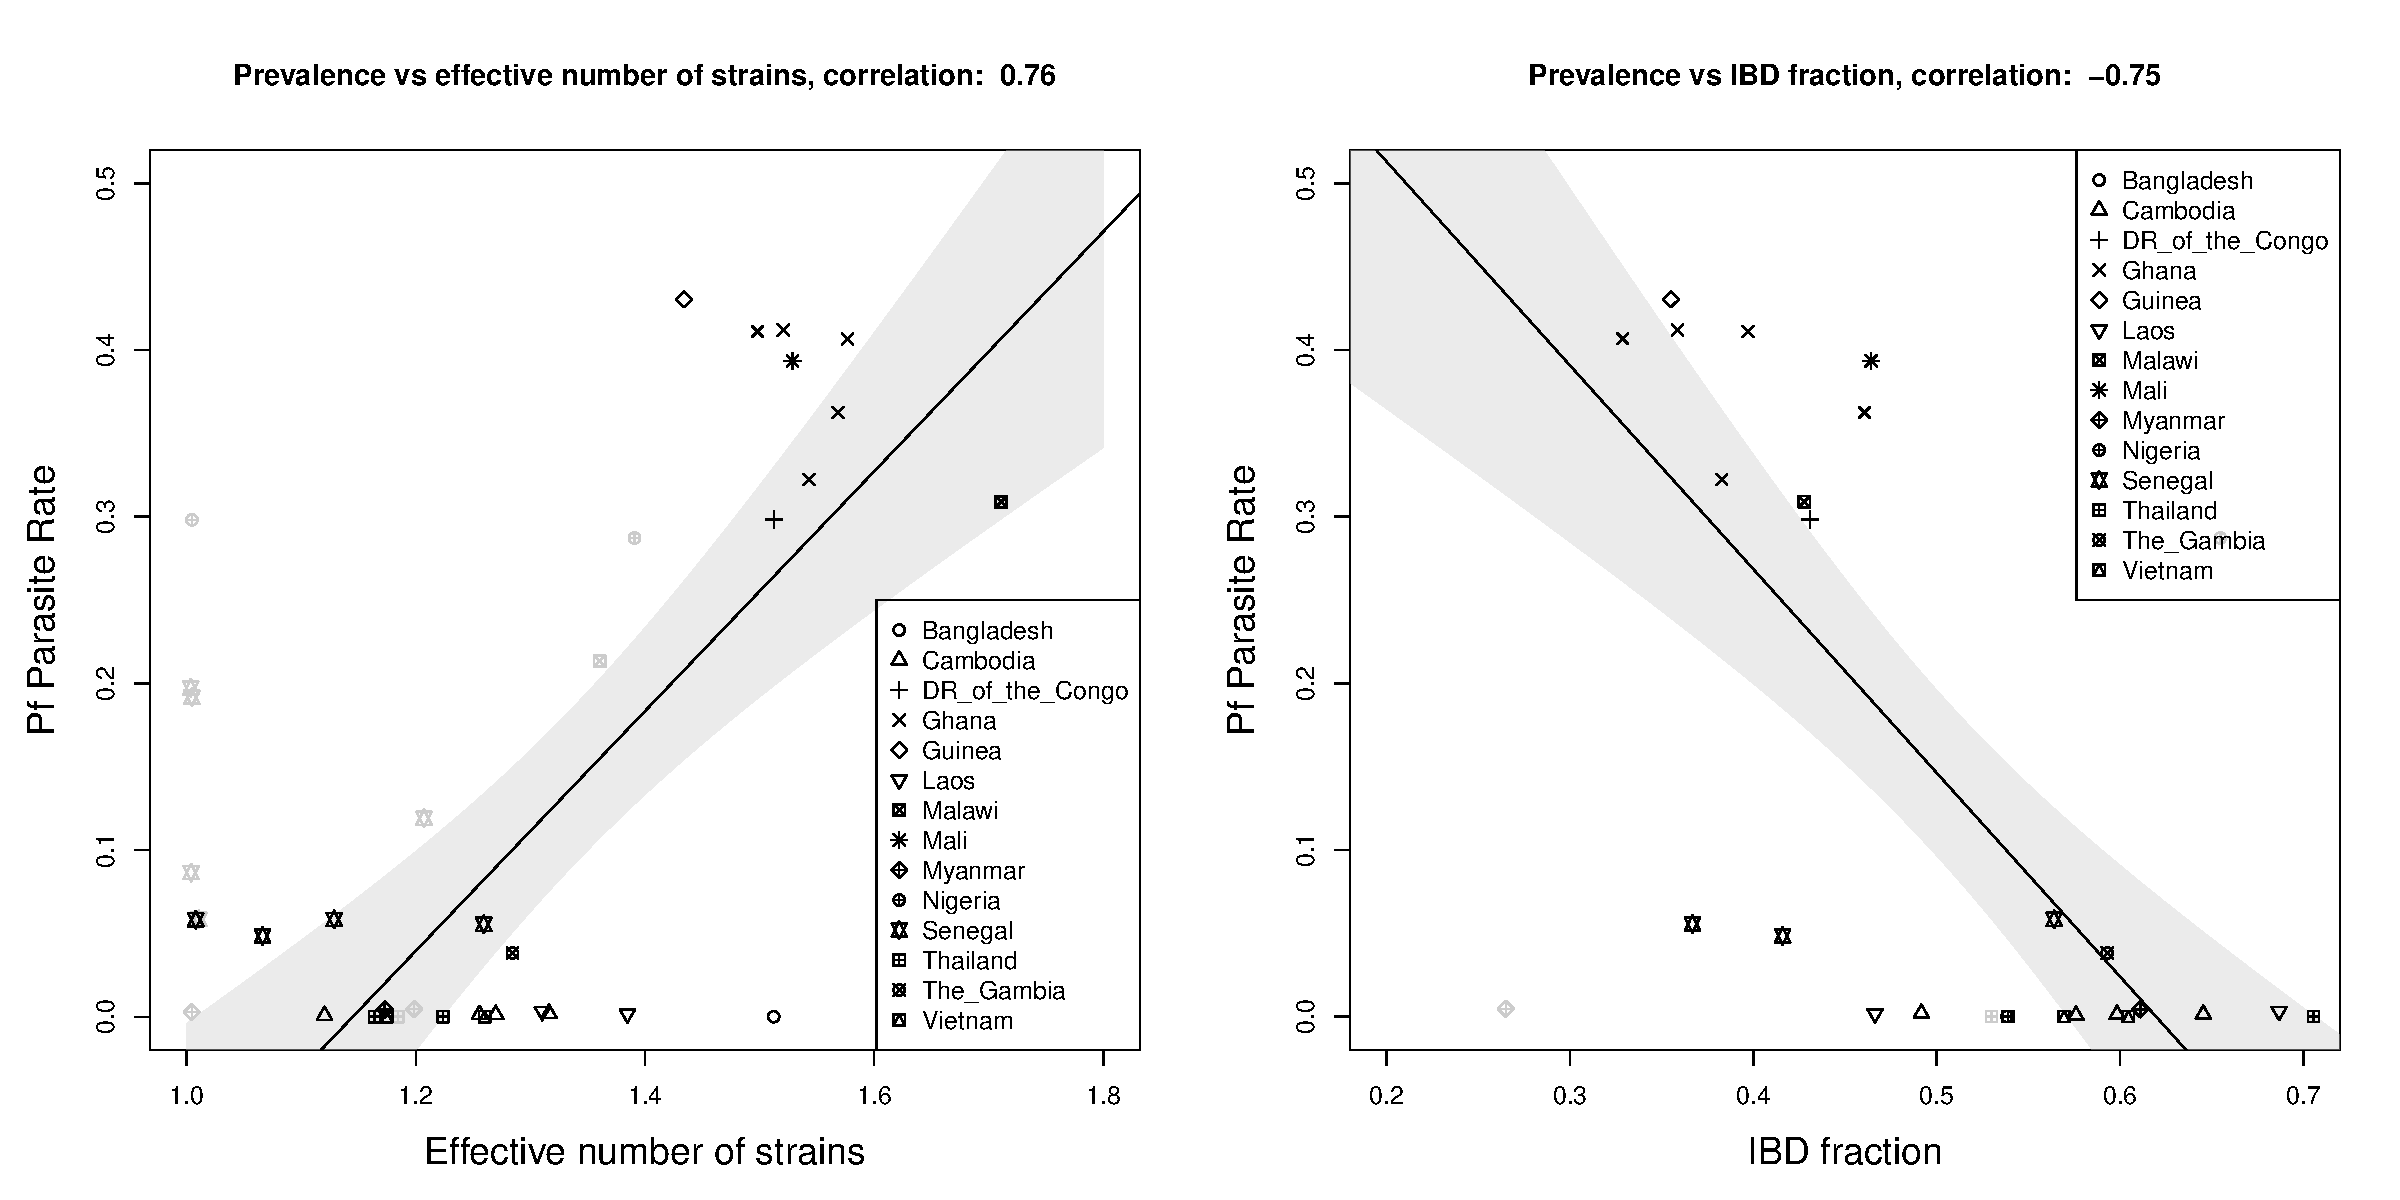
\includegraphics[width=0.8\textwidth]{prevelance.pdf}
}
%\\
  %\subfloat[][]{
  %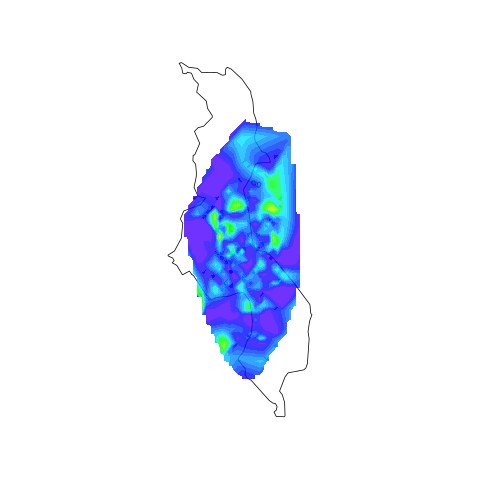
\includegraphics[width=0.8\textwidth]{Malawi.png}
%}
\caption{Black dots show African samples for modelling, red dots are the predicted values \textcolor{red}{1. update with vivax, 2. replace Malawi map with Africa map and Asia map}}
\end{figure}





\section{Discussion}




\section{ACKNOWLEDGMENTS}
We thank the Pf3k consortium for valuable insights. The project is funded by  Wellcome (100956/Z/13/Z to GM, \ldots).




\section{DISCLOSURE DECLARATION}
None declared.





\bibliography{mixedIBD.bib}


\end{document}
